%作者:汪斐然
%模板用途:模式识别报告
%时间:2021年3月

%这是一份基于《2020-2021模式识别期末提交模板》Word版制作的Latex模板。用于方昱春老师的模式识别课程报告。
%文档中对Latex的各种使用方式都准备了样例并进行备注,包括标题设置、图表添加、文献引用以及字体设置等。
%参考文献格式和Word版存在一定的区别,使用的是IEEETR格式。是IEEE期刊使用的参考文献引用标准。
%参考文献选择使用IEEETR格式的原因在于,可以在文章中对参考文献进行超链接索引。
%希望这份模板可以帮助同学们快速上手Latex,制作漂亮的课程报告;可以在同学们之后的研究学习过程中成为学术论文的参考模板。

%Latex工具:本地编辑平台:TexWorks;在线编辑平台:Overleaf(推荐)

%Latex快速入门教程:
%1、https://muyuuuu.github.io/2018/11/07/Brief-introduction-to-LaTex/
%2、https://liam.page/2014/09/08/latex-introduction/

%Latex快速辅助工具使用说明:
%快速绘制表格工具:https://www.tablesgenerator.com/
%快速生成公式工具:https://mathpix.com/

%%%%%%%%%%%%%%%%%%%%%%%%%%%%%环境配置%%%%%%%%%%%%%%%%%%%%%%%%%%%%%%%%%%

\documentclass{article}
\usepackage[UTF8]{ctex}
\usepackage[left=3.18cm,right=3.18cm,top=2.54cm,bottom=2.54cm]{geometry}
\geometry{a4paper}

%附录包
\usepackage{appendix} 
\usepackage{listings}

%代码格式
\usepackage{xcolor}
\lstset{
    numbers=left, 
    numberstyle= \tiny, 
    keywordstyle= \color{ blue!70},
    commentstyle= \color{red!50!green!50!blue!50}, 
    frame=shadowbox, % 阴影效果
    rulesepcolor= \color{ red!20!green!20!blue!20} ,
    escapeinside=``, % 英文分号中可写入中文
    xleftmargin=2em,xrightmargin=2em, aboveskip=1em,
    framexleftmargin=2em
} 
\usepackage{algorithm}
\usepackage{algpseudocode}
\renewcommand{\algorithmicrequire}{\textbf{Input:}}  % Use Input in the 
\renewcommand{\algorithmicensure}{\textbf{Output:}} % Use Output in the 

%数学
\usepackage{amsmath}
\usepackage{amsthm}

%图片
\usepackage{graphicx} %添加图片

%字体、格式设置
\usepackage{subfigure}
\usepackage{float}
\usepackage{xeCJK}
\renewcommand{\vec}[1]{\boldsymbol{#1}} % 生产粗体向量,而不是带箭头的向量
\usepackage{amssymb}
\usepackage{booktabs} % excel导出的大表格
\usepackage{hyperref}
\usepackage{titlesec}%设置字体的包
\usepackage{multirow}
%可选字体:
% \noindent 中文字体(默认宋体)\\
% \fangsong 中文字体(仿宋) \songti 中文字体(宋体) \lishu 中文字体(隶书) \heiti 中文字体(黑体)\\
% \CJKfamily{zhkai} 中文字体(楷书) \CJKfamily{zhyou} 中文字体(幼圆) \CJKfamily{zhyahei} 中文字体(微软雅黑)\\

%调整图表标题的字体样式
\usepackage{caption}
\captionsetup{font={small,bf}} 

%新定义
\newtheorem{definition}{定义} %中文
\newtheorem{lemma}{引理}
\newtheorem{theorem}{定理}
\DeclareMathOperator{\Ima}{Im}%定义新符号
\DeclareMathOperator{\Rank}{rank}%定义求秩算子



%设置标题,作者
\title{\textbf{基于HOG+SVM与YOLO的路标识别分类}}
\author{
郑力铖(21122873)
}

%%%%%%%%%%%%%%%%%%%%%%%%%%%%%%%正文%%%%%%%%%%%%%%%%%%%%%%%%%%%%%%%%%%
%\songti(宋体)设置全文字体,可改为\heiti(黑体),\fangsong(仿宋)
\begin{document} \songti

% 插入封面
\centerline{\heiti\zihao{2}{上海大学2023 $ \sim $ 2024学年}}
\vspace{10bp}
\centerline{\heiti\zihao{2}{课程报告成绩评价表}}

\vskip 2cm

\begin{flushleft}
    \zihao{3}
    {\heiti{课程名称:}}
    {\heiti\underline{\quad\textbf{《模式识别》}\quad}}
    {\heiti{课程编号:}}
    {\heiti\underline{\quad\textbf{08306089}\hspace{1cm}}}  \\
    \vspace{20bp}
    {\heiti{ {报告名称:}}}
    {\heiti\underline{\quad\textbf{基于HOG+SVM与YOLO的路标识别}\quad}} \\
    \vspace{20bp}
    {\heiti{{姓}\quad\quad{名:}}}
    {\heiti\underline{\quad\quad\textbf{郑力铖}\quad\quad}}
    {\heiti{{学}\quad\quad{号:}}}
    {\heiti\underline{\quad\textbf{21122873}\quad}} \\
    \vspace{20bp}
    {\heiti{ {报告评语:}}} \\
    \vspace{5bp}
    \fbox{
        \parbox{\textwidth}{
            \begin{center}
                \leavevmode \\ \quad
                \leavevmode \\ \quad
                \leavevmode \\ \quad
                \leavevmode \\ \quad
            \end{center}
        }
    }

    \vspace{20bp}
    {\heiti{{报告成绩:}}}
    \\
    \vspace{5bp}
    \begin{table}[htbp]
        \setlength{\tabcolsep}{0.37cm}{
            \begin{tabular}{|cl|cl|cll|c|}
                \hline
                \multicolumn{2}{|c|}{方案设计(20分)}          & \multicolumn{2}{c|}{验收(20分)}              & \multicolumn{3}{c|}{书面报告(60分)}          & \multirow{2}{*}{总分}                                                                                                                                                                                                     \\ \cline{1-7}
                \multicolumn{1}{|c|}{\begin{tabular}[c]{@{}c@{}}可行性\\ (10分)\end{tabular}} & \multicolumn{1}{c|}{\begin{tabular}[c]{@{}c@{}}创新性\\ (10分)\end{tabular}} & \multicolumn{1}{c|}{\begin{tabular}[c]{@{}c@{}}规范性\\ (10分)\end{tabular}} & \multicolumn{1}{c|}{\begin{tabular}[c]{@{}c@{}}演示效果\\ (10分)\end{tabular}} & \multicolumn{1}{c|}{\begin{tabular}[c]{@{}c@{}}规范性\\ (20分)\end{tabular}} & \multicolumn{1}{c|}{\begin{tabular}[c]{@{}c@{}}完整性\\ (20分)\end{tabular}} & \multicolumn{1}{c|}{\begin{tabular}[c]{@{}c@{}}科学性\\ (20分)\end{tabular}} &                       \\ \hline
                \multicolumn{1}{|l|}{}                          &                                                & \multicolumn{1}{l|}{}                          &                                                & \multicolumn{1}{l|}{}                          & \multicolumn{1}{l|}{}                          &                                                & \multicolumn{1}{l|}{} \\ \hline
            \end{tabular}}
    \end{table}
\end{flushleft}

\vspace{20bp}
\leftline{\heiti\zihao{3}{任课教师:}}
\vspace{20bp}
\leftline{\heiti\zihao{3} {评阅日期:     \quad\quad\quad     年  \quad\quad  月  \quad\quad  日         }} %调用封面文件

\date{}
\maketitle


%%%%%%%%%%%%%%%%%%%%%%摘要%%%%%%%%%%%%%%%%%%%%%%%%%%%%%
%由摘要和关键词两部分组成
\begin{center}
    \setlength{\textwidth}{15cm}
    \parbox{\textwidth}{
        \textbf{摘要:}作为交通系统的基本要素,交通标志提供了关于驾驶员、行人等的道路状况的重要信息,来降低事故风险。随着计算机视觉和人工智能的快速发展,交通标志识别算法已被应用于先进的驾驶员辅助系统和自动驾驶系统,以帮助驾驶员和自动驾驶车辆准确获取道路信息。然而在实际应用中,交通标志识别仍然具有挑战性。本文对比了经典的机器学习方法HOG+SVM,和通用视觉识别模型yolov5和yolov8方法,探讨在自动驾驶场景下的路标识别方法。
        \newline
        \textbf{关键词:}图像识别, 支持向量机, 深度学习, 神经网络。
    }
\end{center}

%%%%%%%%%%%%%%%%%%%%%%目录%%%%%%%%%%%%%%%%%%%%%%%%%%%%%
% \newpage
% \tableofcontents
% \newpage
%%%%%%%%%%%%%%%%%%%%%%%%%%%%%%%%%%%%%%%%%%%%%%%%%%%%%%%%
%一级标题
\section{引言}
%%%%%%%%%%%%%%%%%%%%%%%%%%%
%二级标题
\subsection{问题提出}
%三级标题
作为高级驾驶员辅助系统(ADAS)和自动驾驶系统(ADS)的重要组成部分,交通标志识别(TSR)技术可以帮助驾驶员和自动驾驶汽车获取重要的道路信息\cite{chen2022realtime}。交通标志识别TSR是一种为自动驾驶车辆识别道路上的交通标志的智能识别系统,是物体检测的一个子任务,类似于人脸识别。

TSR系统通常由检测和分类两个阶段组成。检测通常使用形状和颜色来识别交通标志的特征,从而从自然场景中提取交通标志。更好的分类能更准确地识别的内容检测到的交通信号。交通标志的识别度,对于避免道路事故具有重大意义\cite{Zhang2017}。本文通过对比不同方法的实际应用效果,旨在为自动驾驶系统选择最合适的路标识别方法提供参考。考虑到实时性、准确性和鲁棒性等因素,读者将能够更好地了解何种方法在特定条件下更为适用。

%%%%%%%%%%%%%%%%%%%%%%%%%%%
\subsection{求解方案分析}
一般来说,交通标志识别有两种检测方法,一种是传统方法(人工定制的特征),另一种是深度学习方法(学习具有深度神经网络的特征)。对于传统方法而言,整个实现流程通常包括的提取区域兴趣(包括交通标志),提取特征(例如HOG),以及然后将这些特征发送到分类器(例如SVM)。然而,传统方法在多类任务中的表现的性能较差。近年来,深度学习方法在许多任务中表现出优异的性能,例如图像分类和检测。对于对象检测,深度学习方法(例如YOLO\cite{ref9},Faster R-CNN\cite{Ren2016})在主流基准上表现良好,准确度和速度都较传统方法有较大优势。

早在 2005 年,方向梯度直方图(HOG)就被提出,HOG用来提取图片特征,并和支持向量机(SVM)结合,最早用来进行行人检测。HOG+SVM这种经典的机器学习方法在过去取得了一定的成功,但随着技术的进步,人们开始寻求更加高效、准确的解决方案。近年来,YOLO算法以其高速度和高精度迅速走红。因此,本文深入研究了yolov5和yolov8这两种先进的目标检测模型。这两种模型都是基于yolo模型的优化,利用深度学习技术,通过神经网络层次结构和先进的目标检测算法,在图像中快速准确地识别路标。相较于传统方法,它们在处理复杂场景和多类别标识时表现更为出色。

%%%%%%%%%%%%%%%%%%%%%%%%%%%
\subsection{论文概述}
本文的其余部分的组织如下。在第二章我们介绍了梯度直方图与支持向量机(HOG+SVM),以及对象检测算法YOLO的算法概述。在第三章我们实现了HOG+SVM,YOLOv5和YOLOv8在数据集上的实验代码,介绍了算法的总体框架,并做了一部分改进。第四章分别对HOG+SVM,和YOLO的两种算法进行了对比,同时在YOLOv5和YOLOv8间的实验结果做了对比。最后在第五章做了讨论和结论。

%%%%%%%%%%%%%%%%%%%%%%%%%%%%%%%%%%%%%%%%%%%%%%%%%%%%%%%%
\section{相关算法概述}
%%%%%%%%%%%%%%%%%%%%%%%%%%%
\subsection{梯度直方图(HOG)}
梯度直方图(Histogram of oriented gradient,简称HOG)\cite{1467360}是应用在计算机视觉和图像处理领域,用于目标检测的特征描述器。这项技术是用来计算局部图像梯度的方向讯息的统计值。在HOG特征描述符中,梯度方向的分布,也就是梯度方向的直方图被视作特征。图像的梯度(x和y导数)非常有用,因为边缘和拐角(强度突变的区域)周围的梯度幅度很大,并且边缘和拐角比平坦区域包含更多关于物体形状的信息。方向梯度直方图(HOG)特征描述符常和线性支持向量机(SVM)配合使用,用于训练高精度的目标分类器。

\subsection{支持向量机(SVM)}
支持向量机(Support Vector Machine,常简称为SVM,又名支持向量网络)\cite{708428}是在分类与回归分析中分析数据的监督式学习模型与相关的学习算法。给定一组训练实例,每个训练实例被标记为属于两个类别中的一个或另一个,SVM训练算法创建一个将新的实例分配给两个类别之一的模型,使其成为非概率二元线性分类器。SVM模型是将实例表示为空间中的点,这样映射就使得单独类别的实例被尽可能宽的明显的间隔分开。然后,将新的实例映射到同一空间,并基于它们落在间隔的哪一侧来预测所属类别。

\subsection{对象检测算法YOLO}
YOLO(You Only Look Once)\cite{ref9}是一种流行的对象检测和图像分割模型,由华盛顿大学的Joseph Redmon和Ali Farhadi开发。它的主要特点是在一次前向传递中,同时完成对象定位和分类。相较于传统的对象检测方法,YOLO在速度和准确性上取得了很大的突破。这使得它适用于实时目标检测任务,如视频分析和自动驾驶。


%%%%%%%%%%%%%%%%%%%%%%%%%%%%%%%%%%%%%%%%%%%%%%%%%%%%%%%%
\section{算法实现描述}


\subsection{算法总体框架(>500字)}


\subsection{改进一及分析(>500字)}

\subsection{改进二及分析(>500字)}



%%%%%%%%%%%%%%%%%%%%%%%%%%%%%%%%%%%%%%%%%%%%%%%%%%%%%%%%
\section{实验描述}
\subsection{实验数据和实验方案 (>500字)}


\subsection{实验一及结果分析 (>500字)}

\begin{table}[htpb]
    \caption{HOG+SVM的路标识别多指标分析}
    \begin{center}\label{table:score}
        % \begin{tabularx}{\linewidth}{|c|X|X|X|}
        \begin{tabular}{|c|r|r|r|}
            \hline
                 & \multicolumn{1}{c|}{精确率} & \multicolumn{1}{c|}{召回率} & \multicolumn{1}{c|}{F1得分} \\ \hline
            直行标志 & \quad0.3706\quad\quad& \quad0.3251\quad\quad& \quad0.3464\quad\quad\\ \hline
            左转标志 & \quad0.5889\quad\quad& \quad0.3869\quad\quad& \quad0.4670\quad\quad\\ \hline
            右转标志 & \quad0.3750\quad\quad& \quad0.4565\quad\quad& \quad0.4118\quad\quad\\ \hline
            禁止鸣笛 & \quad0.4999\quad\quad& \quad0.5682\quad\quad& \quad0.5319\quad\quad\\ \hline
            人行横道 & \quad0.8095\quad\quad& \quad0.5965\quad\quad& \quad0.6869\quad\quad\\ \hline
            禁止通行 & \quad0.7288\quad\quad& \quad0.7049\quad\quad& \quad0.7167\quad\quad\\ \hline
        \end{tabular}
    \end{center}
\end{table}
\begin{figure}[thbp!]
    \centering
    \begin{minipage}[t]{0.49\linewidth}
        \centering
        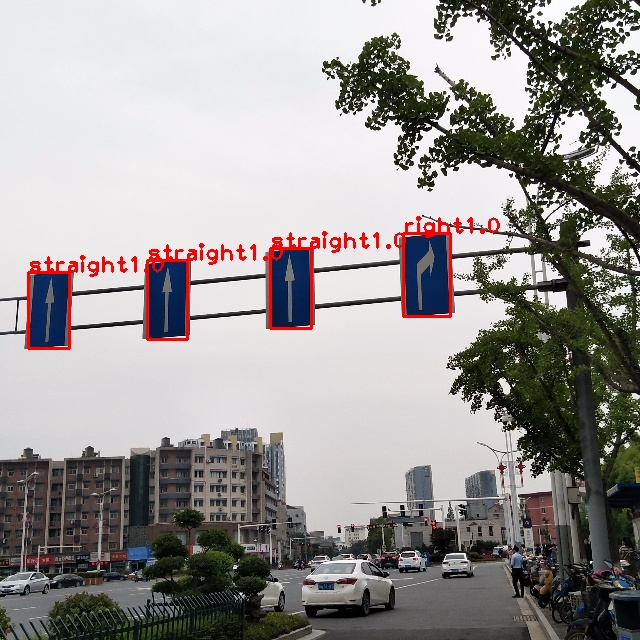
\includegraphics[width=1\linewidth, trim=0 50 0 50, clip]{test_results/sign_433_result.jpg}
        \caption{质量较好的HOG+SVM检测结果}
        \label{fig:1}
    \end{minipage}
    \begin{minipage}[t]{0.49\linewidth}
        \centering
        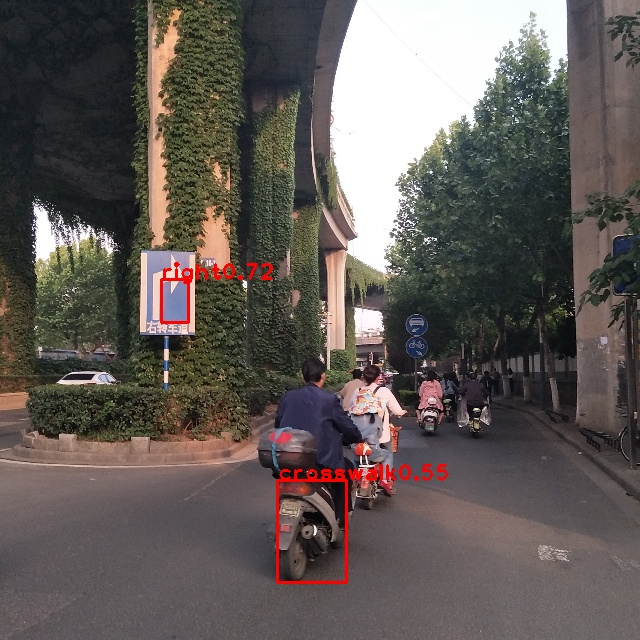
\includegraphics[width=1\linewidth, trim=50 30 50 160, clip]{test_results/sign_120_result.jpg}
        \caption{明显错检与roi不一致问题}
        \label{fig:2}
    \end{minipage}
 \end{figure}

\subsection{实验二及结果分析 (>500字)}

\begin{figure}[htpb]
    \centering
    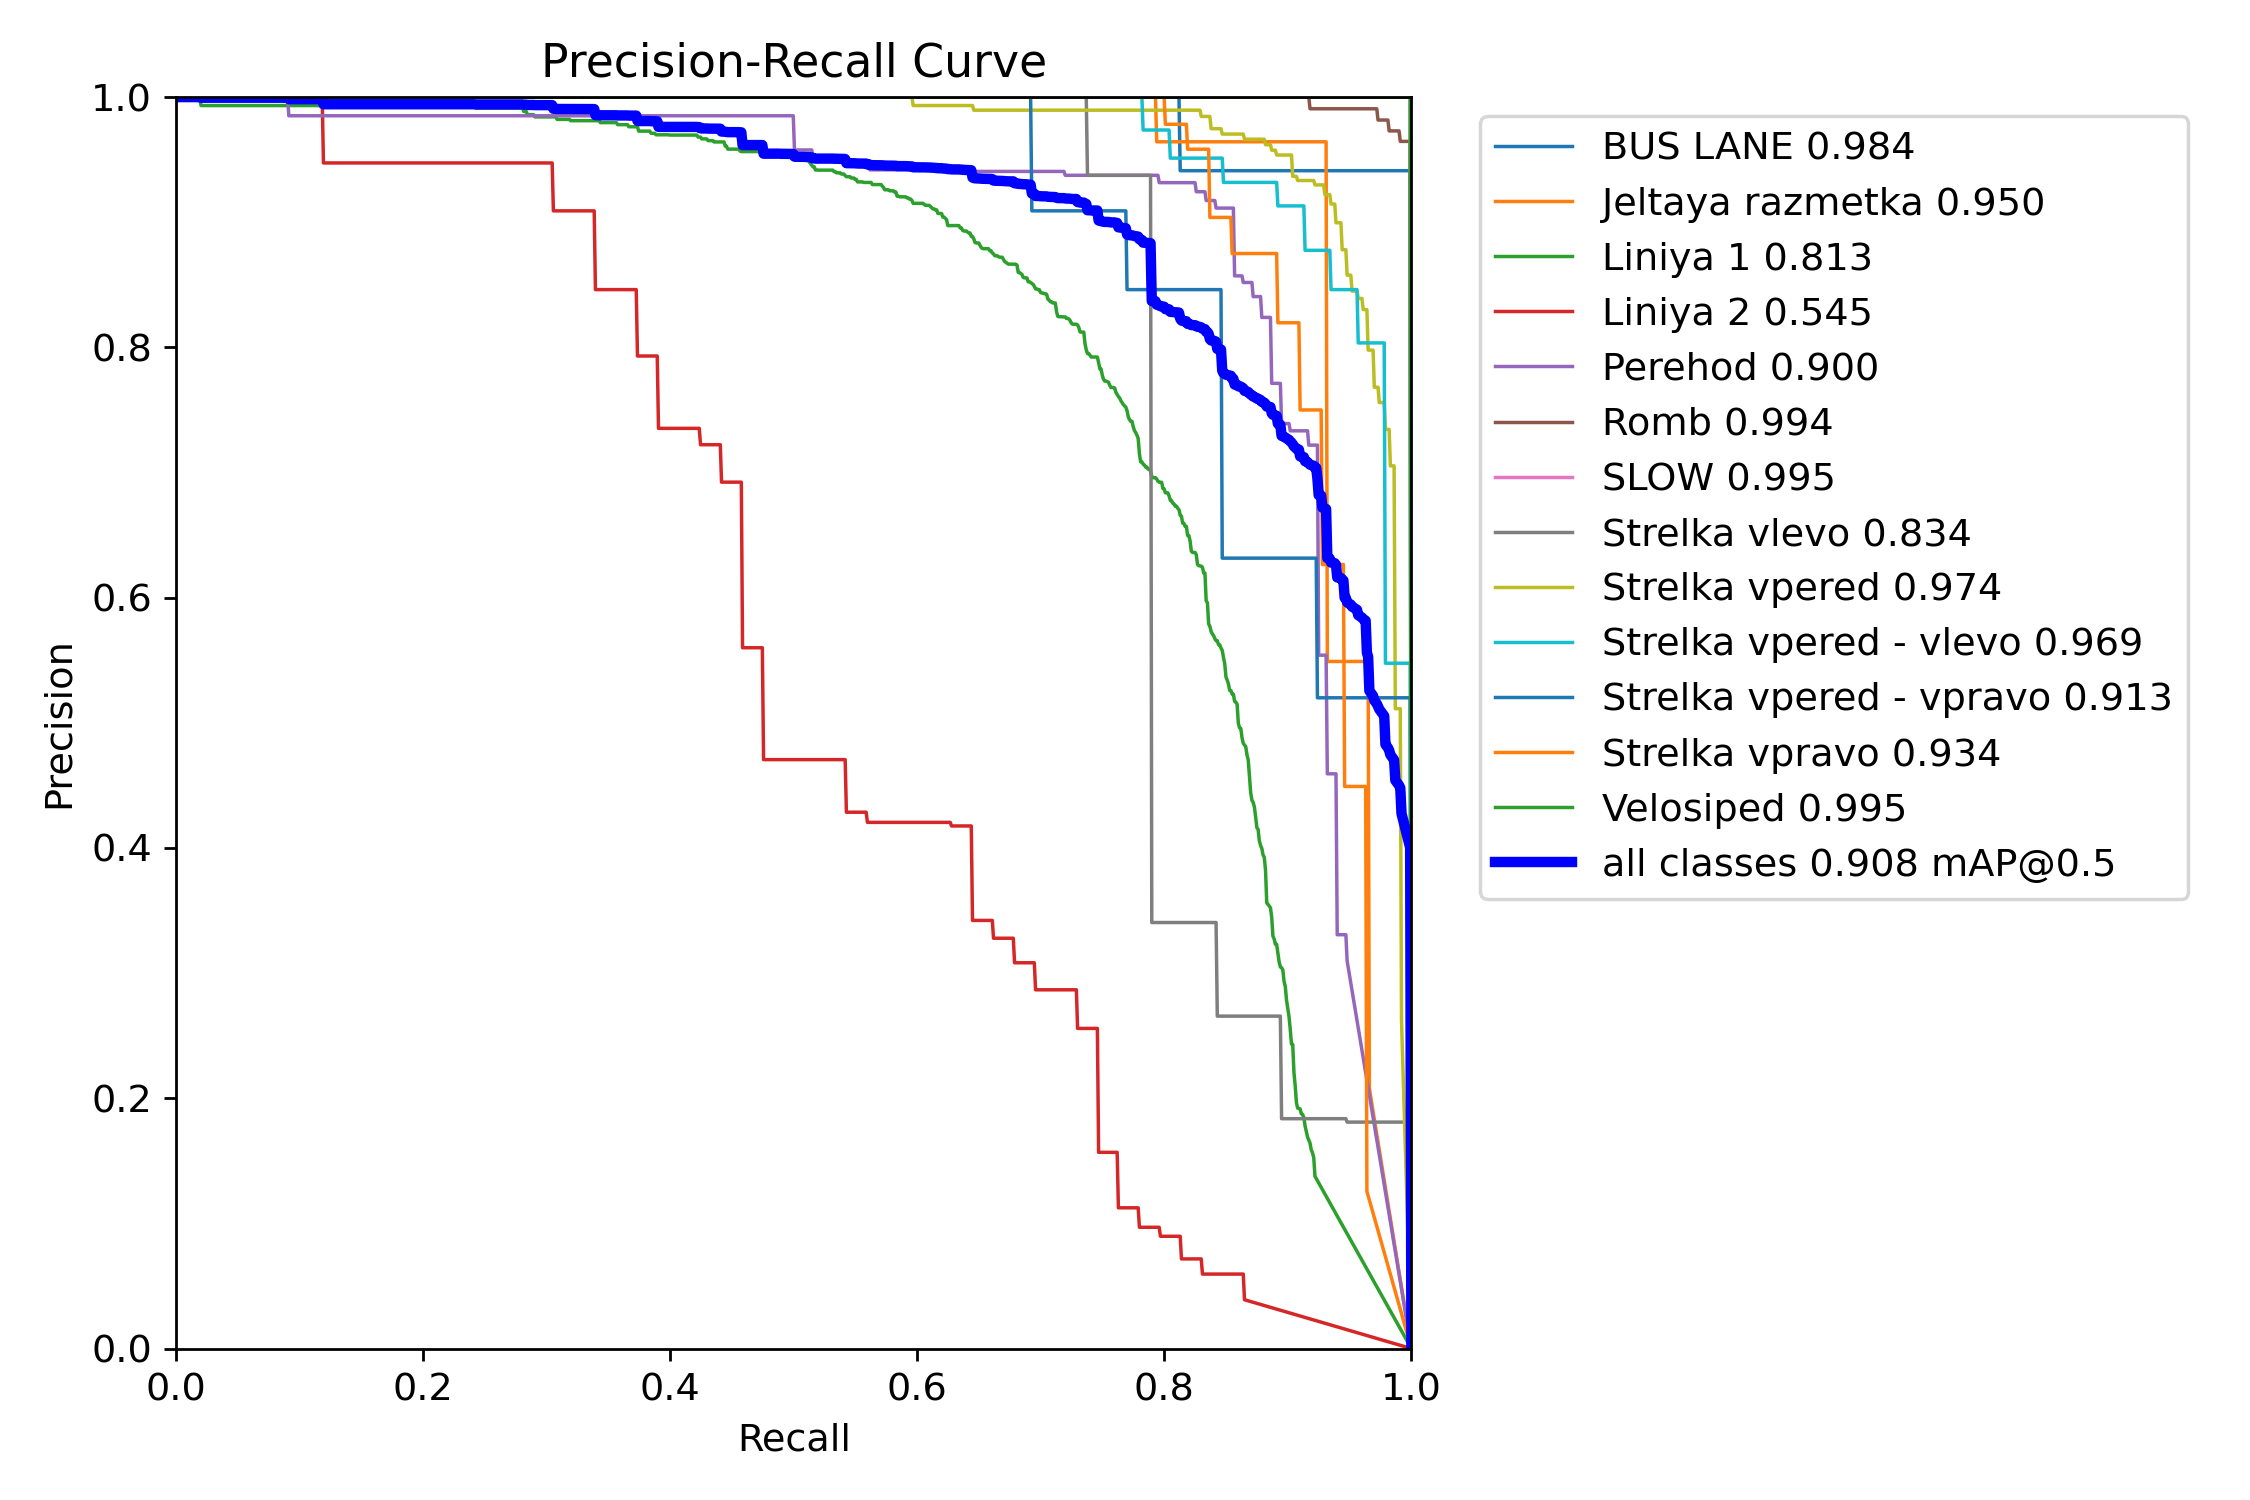
\includegraphics[width=0.9\textwidth]{YOLOv5/train_yolov5/PR_curve.png}
    \caption{YOLOv5的准确度-召回率图,YOLOv8与之类似。}
    \label{fig:3}
\end{figure}


\begin{figure}[htpb]
    \centering
    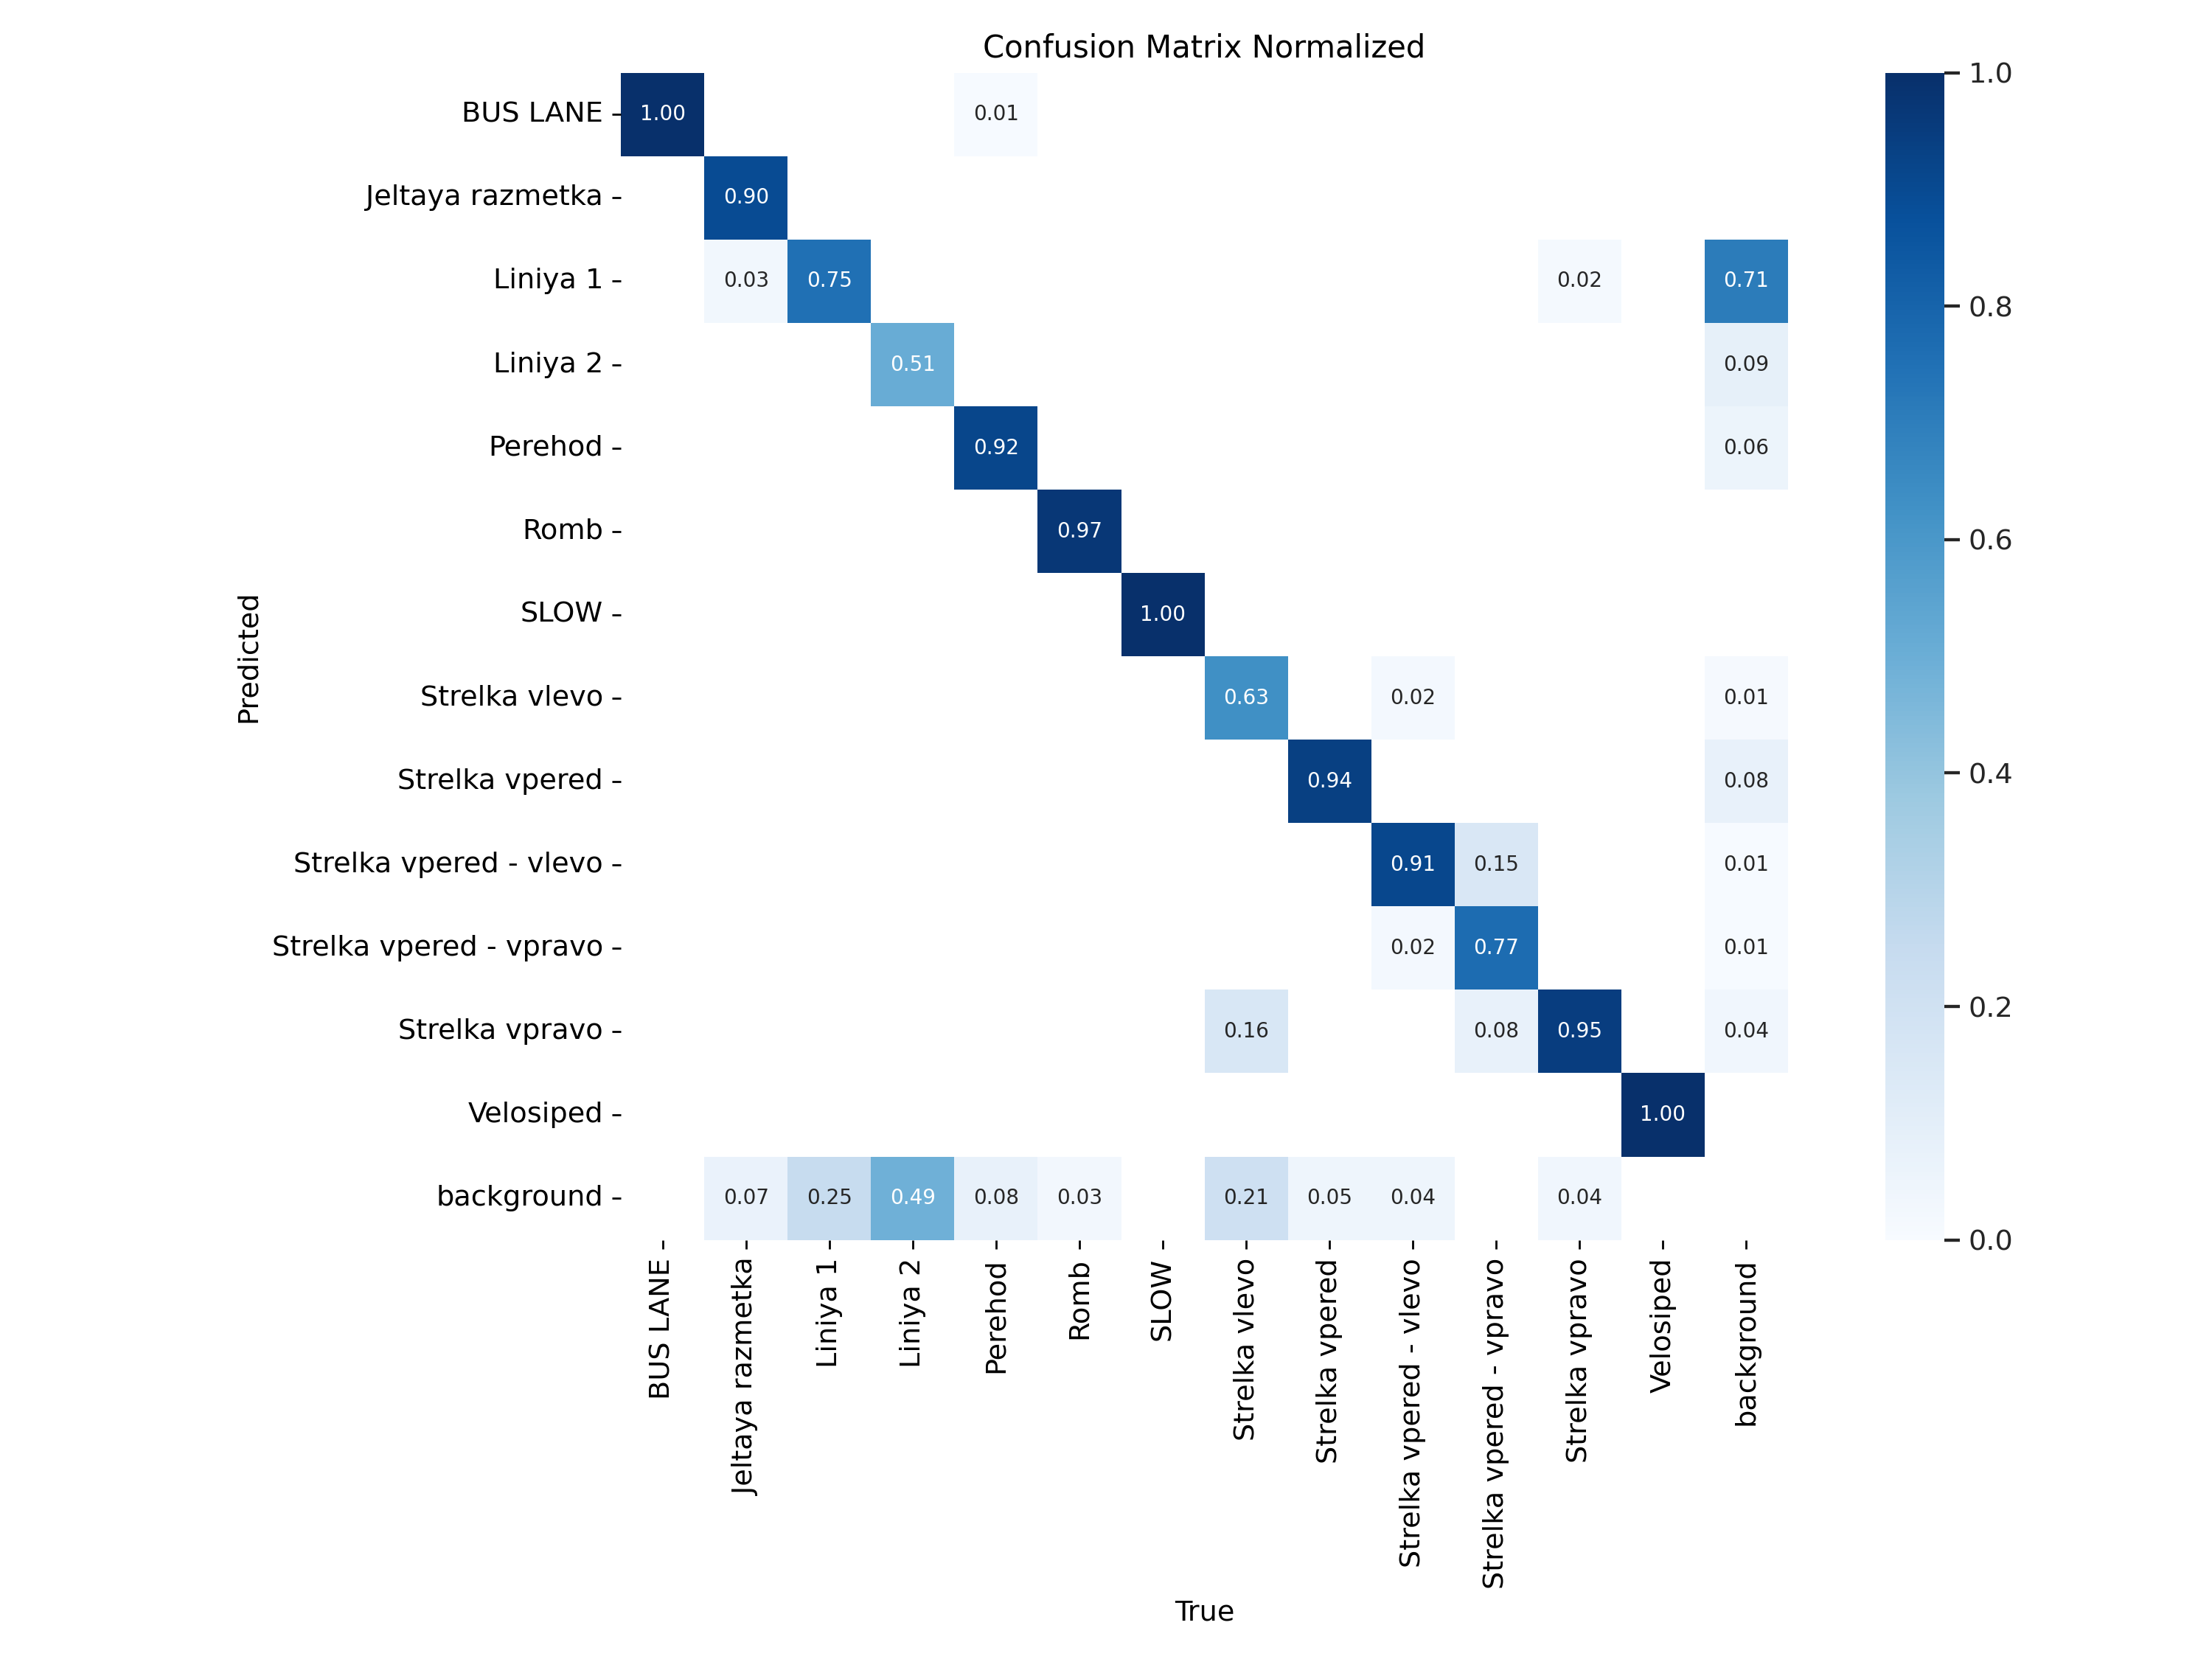
\includegraphics[width=1\textwidth]{YOLOv5/train_yolov5/confusion_matrix_normalized.png}
    \caption{YOLOv5的归一化混淆矩阵图,YOLOv8与之类似。}
    \label{fig:4}
\end{figure}

%%%%%%%%%%%%%%%%%%%%%%%%%%%%%%%%%%%%%%%%%%%%%%%%%%%%%%%%
\section{结论(500字)}


%%%%%%%%%%%%%%%%%%%%%%%%%%%%%%%%%%%%%%%%%%%%%%%%%%%%%%%%
\section{学习体会和建议}
本学期在模式识别课上,方昱春老师深入地介绍了一些模式识别的理论基础,与不同算法模型和技术,以及它们在一些不同场景中的应用。建立起一定的理论基础后,通过研讨和小组作业等形式,上手实际项目,让我更好地理解了算法模型的工作原理、优缺点以及如何调整参数以提高性能。这培养了我解决问题的能力,有助于更好地理解问题,从而选择合适的方法,并在实践中更加灵活地应用知识。希望今后能在课程中加入更多前沿领域的最新科研成果分享,并与小组作业有机结合起来,让同学们更好地感受到新成果带来的进步,并能有机会启发同学们在今后参与进前沿的计算机科研的的工作中去的热情。


%%%%%%%%%%%%%%%%%%%引用文献%%%%%%%%%%%%%%%%%%%%%%%%%%%%%%
\bibliography{article}      % 指定article 代表同目录下的article.bib文件 
\bibliographystyle{ieeetr}  % 定义文献引用的格式

%%%%%%%%%%%%%%%%%%%%%%%附录%%%%%%%%%%%%%%%%%%%%%%%%%%%%%%
\newpage{}
\appendix
\section{附录}
\begin{appendices}
    1、图模板
    \begin{figure}[htpb]
        \centering
        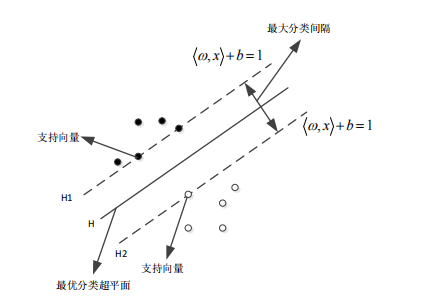
\includegraphics[width=0.5\textwidth]{svm.png}
        \caption{SVM模型原理图}
        \label{fig:svm}
    \end{figure}

    3、公式模板
    \begin{equation}\label{eq:svmsuper}
        \begin{array}{l}
            \min _{\boldsymbol{w}, b} \frac{1}{2}\|\boldsymbol{w}\|^{2} \\
            \text { s.t. } y_{i}\left(\boldsymbol{w}^{\mathrm{T}} \boldsymbol{x}_{i}+b\right) \geqslant 1, \quad i=1,2, \ldots, m
        \end{array}
    \end{equation}


    4、伪代码模板
    \begin{algorithm}[H]
        \caption{ K近邻算法步骤}
        \begin{algorithmic}[1]
            \Require
            训练数据集;
            待预测数据;
            \Ensure
            预测数据的类别;
            \State 加载数据;
            \State 初始化K值;
            \State 计算预测样本与训练集中的每一个样本的距离;
            \State 将距离和索引添加到有序集合中;
            \State 对距离按从小到大排序方式对距离和索引的有序集合进行排序;
            \State 从排序的集合中选择前K条数据;
            \State 获得选的K条数据的标签;
            \State 计算每一种标签的样本数量;
            \Return
            数量最多的标签作为样本的预测值;
        \end{algorithmic}
    \end{algorithm}


    5、核心代码
    \lstset{language=Python}
    \begin{lstlisting}
#调整图片尺寸到统一大小,并扁平化为一维数据
def image_to_feature_vector(image, size=(128, 128)):

	return cv2.resize(image, size).flatten()

#提取图像在HSV颜色空间上的颜色直方图,将直方图扁平化,
#作为特征向量返回
def extract_color_histogram(image, bins=(32, 32, 32)):
	hsv = cv2.cvtColor(image, cv2.COLOR_BGR2HSV)
	hist = cv2.calcHist([hsv], [0, 1, 2], None, bins,
		[0, 180, 0, 256, 0, 256])
	if imutils.is_cv2():
		hist = cv2.normalize(hist)
	else:
		cv2.normalize(hist, hist)
	return hist.flatten()

    \end{lstlisting}
\end{appendices}

\end{document}
